%============================================================
%  Sparse Koopman Autoencoders (SKAE) — 30-minute seminar talk
%  Clean custom Beamer theme (pdflatex-compatible, no external fonts)
%  Unibody (single-column) design: one idea per slide, light text.
%============================================================
\documentclass[aspectratio=169,10pt]{beamer}

\usepackage[T1]{fontenc}
\usepackage{lmodern}
\usepackage{helvet}
\renewcommand{\familydefault}{\sfdefault}
\usepackage{amsmath,amssymb,bm}
\usepackage{graphicx}
\usepackage{booktabs}
\usepackage{array}
\usepackage{xcolor}
\usepackage{tikz}
\usetikzlibrary{arrows.meta,positioning,calc,shapes.geometric,backgrounds,fit,decorations.pathreplacing}

%------------------ palette ------------------
\definecolor{skaeink}{HTML}{1F2A44}
\definecolor{skaeblue}{HTML}{2B3E6E}
\definecolor{skaepurple}{HTML}{6C4AB6}
\definecolor{skaeteal}{HTML}{268B7C}
\definecolor{skaeorange}{HTML}{E8792B}
\definecolor{skaered}{HTML}{B03030}
\definecolor{skaegray}{HTML}{6B7280}
\definecolor{skaelight}{HTML}{EEF1F7}
\definecolor{skaelav}{HTML}{ECE7F7}

%------------------ theme ------------------
\usetheme{default}
% Keep standard (Computer Modern) math fonts so uppercase Greek (\Delta, \Phi, ...)
% render correctly; text stays Helvetica. Without this, Beamer routes math's
% upright "operators" font to the sans text font, which lacks Greek glyphs.
\usefonttheme{professionalfonts}
\useinnertheme{rectangles}
\setbeamercolor{structure}{fg=skaeblue}
\setbeamercolor{normal text}{fg=skaeink}
\setbeamercolor{alerted text}{fg=skaeorange}
\setbeamercolor{title}{fg=skaeink}
\setbeamercolor{frametitle}{fg=skaeblue,bg=white}
\setbeamercolor{itemize item}{fg=skaepurple}
\setbeamercolor{itemize subitem}{fg=skaeteal}
\setbeamercolor{enumerate item}{fg=skaepurple}
\setbeamercolor{block title}{fg=white,bg=skaeteal}
\setbeamercolor{block body}{fg=skaeink,bg=skaelight}
\setbeamercolor{block title alerted}{fg=white,bg=skaeorange}
\setbeamercolor{block body alerted}{fg=skaeink,bg=skaelight}
\setbeamercolor{block title example}{fg=white,bg=skaepurple}
\setbeamercolor{block body example}{fg=skaeink,bg=skaelav}

\setbeamerfont{frametitle}{series=\bfseries,size=\Large}
\setbeamerfont{title}{series=\bfseries}
\setbeamerfont{block title}{series=\bfseries}

\setbeamertemplate{navigation symbols}{}
\setbeamertemplate{itemize items}[circle]
\setbeamertemplate{blocks}[rounded][shadow=false]

% frame title: bold blue with rule underneath
\setbeamertemplate{frametitle}{%
  \vspace*{0.55em}%
  {\usebeamerfont{frametitle}\usebeamercolor[fg]{frametitle}\insertframetitle}%
  \ifx\insertframesubtitle\empty\else
    \\[0.1em]{\normalsize\color{skaegray}\insertframesubtitle}%
  \fi
  \vspace*{0.15em}\par
  {\color{skaeblue}\hrule height 1.1pt}%
  \vspace*{0.2em}%
}

% footline
\setbeamertemplate{footline}{%
  \hbox{%
    \begin{beamercolorbox}[wd=.5\paperwidth,ht=2.4ex,dp=1.2ex,leftskip=1.2em]{}%
      {\color{skaegray}\footnotesize Sparse Koopman Autoencoders}%
    \end{beamercolorbox}%
    \begin{beamercolorbox}[wd=.5\paperwidth,ht=2.4ex,dp=1.2ex,rightskip=1.2em]{}%
      \hfill{\color{skaegray}\footnotesize \insertframenumber\,/\,\inserttotalframenumber}%
    \end{beamercolorbox}%
  }%
  \vspace*{0.2em}%
}

% section divider pages
\AtBeginSection[]{%
  \begin{frame}[plain]
    \centering
    \vfill
    {\color{skaeblue}\rule{0.5\textwidth}{1.4pt}}\\[0.9em]
    {\usebeamerfont{title}\Large\color{skaeink}\insertsectionhead}\\[0.7em]
    {\color{skaeblue}\rule{0.5\textwidth}{1.4pt}}
    \vfill
  \end{frame}
}

%------------------ helper commands ------------------
\newcommand{\takeaway}[1]{%
  \begin{beamercolorbox}[wd=\textwidth,sep=8pt,rounded=true]{block title alerted}%
    \centering\bfseries #1%
  \end{beamercolorbox}}
\newcommand{\emphc}[1]{{\color{skaeorange}\bfseries #1}}
\newcommand{\emphp}[1]{{\color{skaepurple}\bfseries #1}}
\newcommand{\empht}[1]{{\color{skaeteal}\bfseries #1}}
\newcommand{\R}{\mathbb{R}}

% big centered statement slide body
\newcommand{\statement}[1]{\vfill\begin{center}\Large\color{skaeink}#1\end{center}\vfill}
% spaced, larger single-column bullets
\newenvironment{points}{\large\begin{itemize}\setlength{\itemsep}{0.85em}}{\end{itemize}}
% one-line figure caption
\newcommand{\figcap}[1]{\vspace{0.3em}{\small\color{skaegray}#1}}

% ---- EDIT HERE: author list (presenter underlined) ----
\newcommand{\presenter}{Aidan Li, Uday Kiran Reddy Tadipatri, Mahan Fathi, Sarath Chandar, Ross Goroshin}

%============================================================
\begin{document}

%------------------ TITLE ------------------
\begin{frame}[plain]
  \vfill
  \begin{center}
    {\usebeamerfont{title}\LARGE\color{skaeink} Sparse Koopman Autoencoders Identify\\[0.35em]
     Local Dynamical Regimes in Multibasin Systems}\\[1.4em]
    {\color{skaeblue}\rule{0.5\textwidth}{1.1pt}}\\[1.4em]
    {\normalsize\color{skaeink} \presenter}
  \end{center}
  \vfill
  \begin{center}
    $\vcenter{\hbox{\includegraphics[height=1.15cm]{figs/logo_chandarlab_crop.png}}}\hspace{0.75cm}
     \vcenter{\hbox{\includegraphics[height=1.05cm]{figs/logo_mila_purple_crop.png}}}\hspace{0.75cm}
     \vcenter{\hbox{\includegraphics[height=1.42cm]{figs/logo_udem_crop.png}}}$
  \end{center}
  \vspace{0.7em}
\end{frame}

%------------------ ROADMAP ------------------
\begin{frame}{Roadmap}
  \vfill
  \begin{points}
    \item[\textbf{1.}] \textbf{Motivation:} linearizing nonlinear dynamics
    \item[\textbf{2.}] \textbf{Problem:} why multibasin systems break it
    \item[\textbf{3.}] \textbf{Idea:} sparse supports as regime variables
    \item[\textbf{4.}] \textbf{Model:} SKAE and its training
    \item[\textbf{5.}] \textbf{Experiments:} forecasting, interventions, basins
    \item[\textbf{6.}] \textbf{Discussion \& outlook}
  \end{points}
  \vfill
\end{frame}

%============================================================
\section{Motivation: Koopman learning}
%============================================================

%--- the goal ---
\begin{frame}{Objective}
  \statement{Embed nonlinear dynamics into coordinates where the\\ evolution is \emphp{linear}, or at least locally linear.}
  \begin{center}
    \includegraphics[width=0.62\linewidth]{figs/azencot_koopman.png}
  \end{center}
  \figcap{Figure from Azencot et al.\ (2020).}
\end{frame}

%--- why ---
\begin{frame}{Motivation for linear coordinates}
  \vfill
  \begin{points}
    \item Linear models make prediction, estimation, and control easier
    \item A suitable change of coordinates can substantially simplify analysis
  \end{points}
  \vfill
\end{frame}

%--- theory + catch ---
\begin{frame}{Existence results for linearizing coordinates}
  \vfill
  \begin{points}
    \item Local linearization near hyperbolic fixed points (Hartman--Grobman)
    \item Koopman eigenfunctions linearize on a basin of attraction...
    % \item \hfill{\small\color{skaegray}(stable equilibria, periodic orbits)}
  \end{points}
  \begin{center}
  {\Large\color{skaeink}\bfseries but only \emph{existentially}.}\\[0.4em]
  {\large\color{skaeink} Good linear coordinates can exist, but how to build them from finite data?}
  \end{center}
\end{frame}

%--- data-driven route ---
\begin{frame}{A data-driven approach}
  \statement{Rather than hand-designing observables,\\ \emphp{learn} the embedding directly from trajectory data.}
  \begin{center}
    \large DMD\ \ $\to$\ \ eDMD\ \ $\to$\ \ \emphp{Koopman autoencoders}
  \end{center}
  \vfill
\end{frame}

%--- koopman operator ---
\begin{frame}{Koopman operator theory}
  \begin{center}
  Lift the nonlinear map to a \emphp{linear} operator on \emph{observables} $g:\mathcal{X}\to\R$:
  \[
    \Large (\mathcal{K}g)(x)=g\big(F_{\Delta t}(x)\big)
  \]
  \end{center}
  \begin{center}
  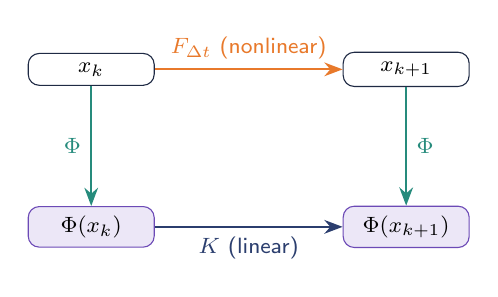
\begin{tikzpicture}[font=\footnotesize,>=Stealth]
    \node[draw=skaeink,rounded corners,fill=white,minimum width=1.6cm] (x0) at (0,0) {$x_k$};
    \node[draw=skaeink,rounded corners,fill=white,minimum width=1.6cm] (x1) at (4.0,0) {$x_{k+1}$};
    \node[draw=skaepurple,rounded corners,fill=skaelav,minimum width=1.6cm] (z0) at (0,-2) {$\Phi(x_k)$};
    \node[draw=skaepurple,rounded corners,fill=skaelav,minimum width=1.6cm] (z1) at (4.0,-2) {$\Phi(x_{k+1})$};
    \draw[->,skaeorange,thick] (x0)--(x1) node[midway,above]{$F_{\Delta t}$ (nonlinear)};
    \draw[->,skaeblue,thick] (z0)--(z1) node[midway,below]{$K$ (linear)};
    \draw[->,skaeteal,thick] (x0)--(z0) node[midway,left]{$\Phi$};
    \draw[->,skaeteal,thick] (x1)--(z1) node[midway,right]{$\Phi$};
  \end{tikzpicture}
  \end{center}
  \vspace{0.2em}
  \begin{center}\small\color{skaegray}
  Finite approximation: find $\Phi$ (lift) and $K$ with $\Phi(F_{\Delta t}(x))\approx K\,\Phi(x)$, keeping enough to reconstruct $x$.
  \end{center}
\end{frame}

%--- KAE ---
\begin{frame}{Koopman autoencoders (KAEs)}
  
  \[
    \Large\boxed{\;\hat{x}_{k+h}\;=\;D_\phi\big(K^{h}\,E_\theta(x_k)\big)\;}
  \]
  \vspace{0.4em}
  \begin{center}\small\color{skaegray}
  Learn encoder $E_\theta$, decoder $D_\phi$, and one latent transition $K$ jointly, from trajectory windows.
  \end{center}
\end{frame}

%--- crucial constraint ---
\begin{frame}{A key modeling constraint}
  \statement{The same transition matrix $K$ is applied at \emph{every} rollout step.\\[0.8em]
  State-dependent structure required for prediction must therefore reside in the learned representation \emphp{$z_k$}, not in a supplied regime label.}
\end{frame}

%============================================================
\section{Problem: multibasin systems}
%============================================================

%--- multistability intuition ---
\begin{frame}{Many systems are multistable}
  \vspace{-0.2em}
  \begin{center}\normalsize
  Different initial conditions settle into \emphp{different} long-run behaviors.
  \end{center}
  \begin{center}
    \includegraphics[height=0.62\textheight,keepaspectratio]{figs/duffing_basins.png}
  \end{center}
  \figcap{Two wells, two shaded basins: where a trajectory \emph{starts} decides which attractor it spirals into.}
\end{frame}

%--- phase portraits (figure, unibody) ---
\begin{frame}{Coexisting attractors partition state space}
  \begin{center}
    \includegraphics[width=0.96\linewidth]{figs/fig1_top_supportbasin.png}
  \end{center}
  \figcap{Procedurally generated 2-D multibasin flows. Gray streamlines = true field; colors = distinct basins.}
\end{frame}

%--- the wall ---
\begin{frame}{An impossibility result}
  \vfill
  \begin{center}
  \begin{beamercolorbox}[wd=0.92\textwidth,sep=14pt,rounded=true]{block title alerted}
    \centering\large\bfseries
    Multibasin systems \emph{cannot generally} admit a single\\
    finite-dimensional \emph{global} linearization with a\\
    continuous encoder--decoder pair.
  \end{beamercolorbox}
  \end{center}
  \vspace{0.5em}
  \begin{center}\small\color{skaegray} (Established in theory; confirmed empirically.)\end{center}
  \vfill
\end{frame}

%--- reframe ---
\begin{frame}{Reframing the objective}
  \statement{Rather than forcing all basins through a \emph{single} global linearization,\\[0.6em]
  \emphp{we seek distinct \emph{local} linearizations.}}
\end{frame}

%============================================================
\section{Idea: sparse supports as regime variables}
%============================================================

%--- two things ---
\begin{frame}{Two quantities the representation must encode}
  \vfill
  \begin{points}
    \item[\emphp{(i)}] \textbf{Which} local linearization is active
    \item[] \hspace{1.6em}{\normalsize\color{skaegray} a \emph{discrete} regime label}
    \item[\empht{(ii)}] \textbf{Coordinates} that linearize dynamics within it
    \item[] \hspace{1.6em}{\normalsize\color{skaegray} a \emph{continuous} local chart}
  \end{points}
  \vfill
\end{frame}

%--- sparse gives both ---
\begin{frame}{A sparse code encodes both quantities}
  \vspace{0.4em}
  \begin{center}\large
  the \emphp{support} (active coordinates) $\;\Rightarrow\;$ \emph{which} regime\\[0.5em]
  the \empht{nonzero values} $\;\Rightarrow\;$ local Koopman coordinates
  \end{center}
  \vspace{0.6em}
  \begin{center}
  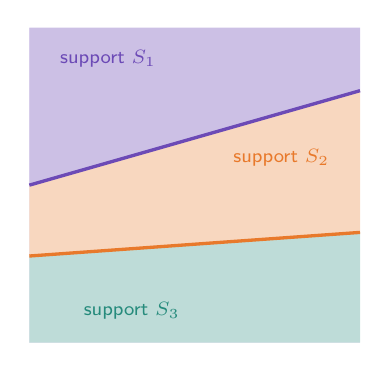
\begin{tikzpicture}[font=\scriptsize]
    \fill[skaelav] (-2.1,-2.0) rectangle (2.1,2.0);
    \fill[skaepurple!35] (-2.1,0) -- (2.1,1.2) -- (2.1,2.0) -- (-2.1,2.0) -- cycle;
    \fill[skaeteal!30]  (-2.1,-2.0) -- (2.1,-2.0) -- (2.1,-0.6) -- (-2.1,-0.9) -- cycle;
    \fill[skaeorange!30] (-2.1,-0.9) -- (2.1,-0.6) -- (2.1,1.2) -- (-2.1,0) -- cycle;
    \draw[skaepurple,very thick] (-2.1,0)--(2.1,1.2);
    \draw[skaeorange,very thick] (-2.1,-0.9)--(2.1,-0.6);
    \node[skaepurple] at (-1.1,1.6) {support $S_1$};
    \node[skaeorange] at (1.1,0.35) {support $S_2$};
    \node[skaeteal] at (-0.8,-1.6) {support $S_3$};
  \end{tikzpicture}
  \end{center}
  \figcap{Different regions activate different latent supports: a union-of-subspaces structure.}
\end{frame}

%--- sparse coding ---
\begin{frame}{Sparse coding}
  \begin{center}
  Given an overcomplete dictionary $D$, find a code with \emphp{few nonzeros}:
  \end{center}
  \vspace{0.5em}
  \[
    \Large z^\star(x)=\arg\min_{z}\ \tfrac12\|x-Dz\|_2^2+\lambda_{\mathrm{sc}}\|z\|_1
  \]
  \vspace{0.6em}
  \begin{center}\large\color{skaegray}
  The $\ell_1$ penalty drives most coordinates to \emph{exactly} zero.
  \end{center}
\end{frame}

%--- LISTA ---
\begin{frame}{Learned ISTA (LISTA): sparse coding as an encoder}
  \begin{center}
  Unroll the iterative solver into a fixed-depth network:\quad $z=E_\theta(x)$
  \end{center}
  \vspace{0.3em}
  \[
    u^{(0)}=\mathrm{shrink}(c,\tau),\qquad u^{(q+1)}=\mathrm{shrink}\!\big(S\,u^{(q)}+c,\tau\big)
  \]
  \begin{center}
  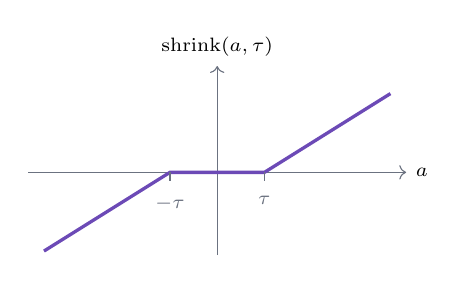
\begin{tikzpicture}[font=\scriptsize]
    \draw[->,skaegray] (-2.4,0)--(2.4,0) node[right,black]{$a$};
    \draw[->,skaegray] (0,-1.05)--(0,1.35) node[above,black]{$\mathrm{shrink}(a,\tau)$};
    \draw[skaepurple,very thick] (-2.2,-1.0)--(-0.6,0)--(0.6,0)--(2.2,1.0);
    \draw[skaegray,dashed] (-0.6,0)--(-0.6,-0.18) node[below]{$-\tau$};
    \draw[skaegray,dashed] (0.6,0)--(0.6,-0.18) node[below]{$\tau$};
  \end{tikzpicture}
  \end{center}
  \figcap{Soft-thresholding zeros out a dead zone $[-\tau,\tau]$, creating the sparse support.}
\end{frame}

%--- why it fits ---
\begin{frame}{The relevant inductive bias}
  \statement{Thresholding makes \emph{exact zeros}.\\[0.6em]
  The encoder \emphp{explicitly selects} active coordinates,\\ and \emph{learns the selection rule} from the prediction objective.}
\end{frame}

%============================================================
\section{The SKAE model \& training}
%============================================================

%--- architecture ---
\begin{frame}{Sparse Koopman Autoencoder (SKAE)}
  \vspace{0.4em}
  \begin{center}
  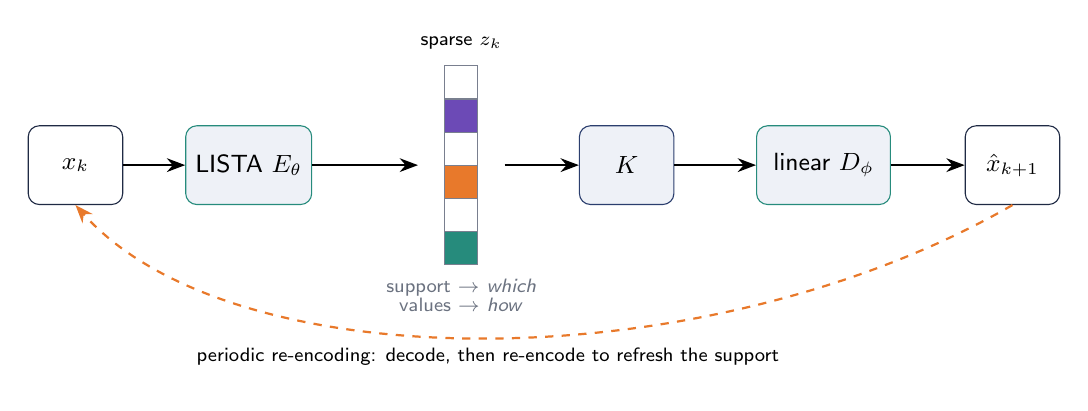
\begin{tikzpicture}[font=\small,>=Stealth]
    \node[draw=skaeink,rounded corners,minimum height=1.0cm,minimum width=1.2cm,fill=white] (x) at (0,0) {$x_k$};
    \node[draw=skaeteal,fill=skaelight,rounded corners,minimum height=1.0cm,minimum width=1.6cm] (E) at (2.2,0) {LISTA $E_\theta$};
    \begin{scope}[shift={(4.9,0)},cell/.style={draw=skaeink!60,minimum width=0.42cm,minimum height=0.42cm}]
      \node[cell,fill=white]      at (0, 1.05) {};
      \node[cell,fill=skaepurple] at (0, 0.63) {};
      \node[cell,fill=white]      at (0, 0.21) {};
      \node[cell,fill=skaeorange] at (0,-0.21) {};
      \node[cell,fill=white]      at (0,-0.63) {};
      \node[cell,fill=skaeteal]   at (0,-1.05) {};
      \node at (0,1.55) {\scriptsize sparse $z_k$};
      \node[skaegray,font=\scriptsize,align=center] at (0,-1.65) {support $\to$ \emph{which}\\[-1pt] values $\to$ \emph{how}};
    \end{scope}
    \node[draw=skaeblue,fill=skaelight,rounded corners,minimum height=1.0cm,minimum width=1.2cm] (K) at (7.0,0) {$K$};
    \node[draw=skaeteal,fill=skaelight,rounded corners,minimum height=1.0cm,minimum width=1.7cm] (D) at (9.5,0) {linear $D_\phi$};
    \node[draw=skaeink,rounded corners,minimum height=1.0cm,minimum width=1.2cm,fill=white] (xh) at (11.9,0) {$\hat{x}_{k+1}$};
    \draw[->,thick] (x)--(E);
    \draw[->,thick] (E)--(4.35,0);
    \draw[->,thick] (5.45,0)--(K);
    \draw[->,thick] (K)--(D);
    \draw[->,thick] (D)--(xh);
    \draw[->,skaeorange,thick,dashed] (xh.south) .. controls (8,-2.75) and (2,-2.75) .. (x.south)
      node[midway,below,black,font=\scriptsize]{periodic re-encoding: decode, then re-encode to refresh the support};
  \end{tikzpicture}
  \end{center}
  \vspace{0.4em}
  \figcap{A LISTA encoder produces a sparse code; a unit-norm linear dictionary decodes; one matrix $K$ advances the latent.}
\end{frame}

%--- two objectives ---
\begin{frame}{Two complementary objectives}
  \vfill
  \begin{points}
    \item \emphp{Koopman:} values on each support evolve \emph{linearly} under $K$
    \item \empht{Sparsity:} different regimes use \emph{different} active coordinates
  \end{points}
  \vfill
  \begin{center}\large\color{skaeink}
  Jointly, the discrete support selects the regime while the\\ continuous values parameterize its local linear dynamics.
  \end{center}
  \vfill
\end{frame}

%--- transition families (visual triptych) ---
\begin{frame}{Three structures for the transition $K$}
  \vspace{0.6em}
  \begin{columns}[T]
    \begin{column}{0.33\textwidth}\centering
      \textbf{Dense}\\[0.5em]
      
\begin{tikzpicture}[scale=0.5]
        \fill[skaeblue!25] (0,0) rectangle (4,4);
        \draw[skaeink] (0,0) rectangle (4,4);
      \end{tikzpicture}\\[0.4em]
      {\footnotesize all coordinates mix}
    \end{column}
    \begin{column}{0.33\textwidth}\centering
      \textbf{Block-diagonal}\\[0.5em]
      
\begin{tikzpicture}[scale=0.5]
        \draw[skaeink] (0,0) rectangle (4,4);
        \fill[skaeteal!35] (0,3) rectangle (1,4);
        \fill[skaeteal!35] (1,2) rectangle (2,3);
        \fill[skaeteal!35] (2,1) rectangle (3,2);
        \fill[skaeteal!35] (3,0) rectangle (4,1);
      \end{tikzpicture}\\[0.4em]
      {\footnotesize $M$ groups, no cross-talk}
    \end{column}
    \begin{column}{0.33\textwidth}\centering
      \textbf{Soft-block}\\[0.5em]
      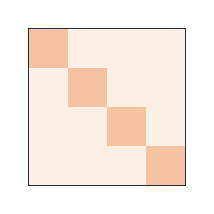
\begin{tikzpicture}[scale=0.5]
        \fill[skaeorange!12] (0,0) rectangle (4,4);
        \fill[skaeorange!45] (0,3) rectangle (1,4);
        \fill[skaeorange!45] (1,2) rectangle (2,3);
        \fill[skaeorange!45] (2,1) rectangle (3,2);
        \fill[skaeorange!45] (3,0) rectangle (4,1);
        \draw[skaeink] (0,0) rectangle (4,4);
      \end{tikzpicture}\\[0.4em]
      {\footnotesize off-block entries penalized}
    \end{column}
  \end{columns}
  \vfill
  \begin{center}\small\color{skaegray}
  Varied \emph{independently} of the encoder, to probe how block structure interacts with learned supports.
  \end{center}
\end{frame}

%--- encoders compared ---
\begin{frame}{Encoders compared}
  \vfill
  \begin{points}
    \item \emphp{LISTA:} sparse \emph{by construction} (thresholding gives exact zeros)
    \item \empht{Sparse MLP:} induced sparsity (ReLU with an $\ell_1$ penalty)
    \item \emphc{Dense MLP:} no sparsity mechanism \hfill {\normalsize\color{skaegray}(control baseline)}
  \end{points}
  \vfill
\end{frame}

%--- training objective ---
\begin{frame}{Training objective: four terms}
  \vfill
  \begin{points}
    \item \emphc{Prediction:} decoded rollout matches future states
    \item \empht{Reconstruction:} code stays tied to the observed state
    \item \emphp{Latent linearity:} rolled-out latent matches encoded latent
    \item \emphp{Sparsity:} few active coordinates
  \end{points}
  \vfill
  \[
    \mathcal{L}=\lambda_{\text{pred}}\bar{\mathcal{L}}_{\text{pred}}
      +\lambda_{\text{rec}}\bar{\mathcal{L}}_{\text{rec}}
      +\lambda_{\text{lin}}\bar{\mathcal{L}}_{\text{lin}}
      +\lambda_{\text{sp}}\bar{\mathcal{L}}_{\text{sp}}
      +\mathcal{L}_{\text{struct}}
  \]
  \vspace{0.2em}
  \begin{center}\small\color{skaegray} No basin labels enter training.\end{center}
\end{frame}

%--- support object 1 ---
\begin{frame}{Support objects (1): the exact support}
  \begin{center}
  Computed \emph{after} training. A Boolean active-coordinate mask:
  \end{center}
  \vspace{0.5em}
  \[
    \Large m_{\mathrm{abs},i}(x)=\mathbf{1}\{|z_i|>10^{-3}\},\qquad
    S_{\mathrm{abs}}=\{i:m_i=1\}
  \]
  \vspace{0.6em}
  \begin{center}\large\color{skaegray}
  Used to test whether the active coordinates are functionally \emph{used}.
  \end{center}
\end{frame}

%--- support object 2 ---
\begin{frame}{Support objects (2): support families}
  \begin{center}
  Group nearby exact supports by \emph{Jaccard overlap} $J(m,r)\ge 0.5$.
  \end{center}
  \vspace{0.2em}
  \begin{center}\small\color{skaegray}
  Jaccard overlap is the \emph{intersection over union} of the two active-coordinate sets:\\[0.3em]
  $\displaystyle J(m,r)=\frac{|\,\mathrm{active}(m)\cap\mathrm{active}(r)\,|}{|\,\mathrm{active}(m)\cup\mathrm{active}(r)\,|}$
  \end{center}
  \vspace{0.3em}
  \begin{center}
  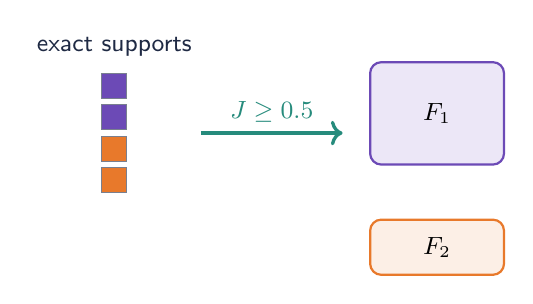
\begin{tikzpicture}[font=\small]
    \node[skaeink] at (-0.5,2.1) {exact supports};
    \foreach \y/\f in {1.6/skaepurple, 1.2/skaepurple, 0.8/skaeorange, 0.4/skaeorange}{
      \node[draw=skaeink!60,minimum size=0.32cm,fill=\f] at (-0.5,\y){};
    }
    \draw[->,skaeteal,very thick] (0.6,1.0)--(2.4,1.0) node[midway,above]{$J\ge 0.5$};
    \node[draw=skaepurple,thick,rounded corners,fill=skaelav,minimum width=1.7cm,minimum height=1.3cm] at (3.6,1.25){$F_1$};
    \node[draw=skaeorange,thick,rounded corners,fill=skaeorange!12,minimum width=1.7cm,minimum height=0.7cm] at (3.6,-0.45){$F_2$};
  \end{tikzpicture}
  \end{center}
  \figcap{Robust, basin-scale objects, with less fragmentation than raw exact supports.}
\end{frame}

%--- two diagnostics ---
\begin{frame}{Two evaluation diagnostics}
  \vfill
  \begin{points}
    \item $H(B\mid F_{\mathrm{abs}})$: uncertainty about the basin given the family
    \item[] \hspace{1.4em}{\normalsize\color{skaegray} \emphp{lower is better}}
    \item $|F_{\mathrm{abs}}|$: number of families
    \item[] \hspace{1.4em}{\normalsize\color{skaegray} compare to the number of basins}
  \end{points}
  \vfill
  \begin{center}\small\color{skaegray} Basin labels are used \emph{only} here, after training, never to train or select the model.\end{center}
  \vfill
\end{frame}

%--- re-encoding ---
\begin{frame}{Periodic re-encoding refreshes the support}
  \vspace{-0.2em}
  \begin{center}\normalsize
  Every $m$ steps the predicted latent is decoded and re-encoded, so the encoder re-selects the active support as the trajectory advances.
  \end{center}
  \begin{center}
    \includegraphics[height=0.57\textheight,keepaspectratio]{figs/reencoding_fathi.png}
  \end{center}
  \figcap{Figure from Fathi et al., ICLR 2024. Squares = ground truth, circles = model-inferred; $\phi,\psi$ are the encoder/decoder (our $E_\theta, D_\phi$).}
\end{frame}

%============================================================
\section{Experiments}
%============================================================

%--- benchmarks ---
\begin{frame}{Benchmarks: 25 systems}
  \vfill
  \begin{points}
    \item \textbf{15 procedural 2-D multibasin systems}
    \item[] \hspace{1em}{\normalsize\color{skaegray} Gaussian wells + rotational drift; \emph{known} basin geometry (eval only)}
    \item \textbf{10 chaotic Dysts flows} ($dt\times 30$)
    \item[] \hspace{1em}{\normalsize\color{skaegray} Chua, Shimizu--Morioka, and more: a long-horizon stress test}
  \end{points}
  \vfill
\end{frame}

%--- six models (grouped list, not a table) ---
\begin{frame}{Six models compared}
  \vfill
  \begin{points}
    \item \emphp{Sparse LISTA encoders}
    \item[] \hspace{1.2em}{\normalsize\color{skaegray} LISTA \textperiodcentered\ LISTA-BD (block-diag.\ $K$) \textperiodcentered\ LISTA-SB (soft-block $K$)}
    \item \empht{Sparse MLP encoders} \hfill {\normalsize\color{skaegray} ReLU $+\ \ell_1$}
    \item[] \hspace{1.2em}{\normalsize\color{skaegray} Sparse MLP \textperiodcentered\ Sparse MLP-BD (block-diag.\ $K$)}
    \item \emphc{Dense MLP} \hfill {\normalsize\color{skaegray} no sparsity: the control baseline}
  \end{points}
  \vfill
\end{frame}

%--- three questions ---
\begin{frame}{Experimental questions}
  \vfill
  \begin{points}
    \item[\textbf{1.}] Do sparse encoders \emph{forecast} better?
    \item[\textbf{2.}] Are the supports \emph{functionally necessary}?
    \item[\textbf{3.}] Do support families \emph{align with basins}?
  \end{points}
  \vfill
\end{frame}

%--- R1 (a): trends ---
\begin{frame}{Result 1: sparse encoders forecast better}
  \begin{center}
    \includegraphics[width=0.9\linewidth]{figs/fig2_forecasting_full.png}
  \end{center}
  \figcap{Held-out MSE, all horizons, both benchmarks. Sparse models improve on the dense baseline at \emph{every} horizon; at $H\!=\!1000$ the dense baseline incurs \emphc{17--27$\times$} higher error.}
\end{frame}

%--- R1 (b): dysts ---
\begin{frame}{Result 1: qualitative behavior on chaotic flows}
  \begin{center}
    \includegraphics[width=0.94\linewidth]{figs/fig1_bottom_dysts.png}
  \end{center}
  \figcap{The \emphc{dense MLP (red)} loses the Chua attractor; the \emphp{LISTA (blue)} forecast stays on the true manifold. \textbf{Sparsity in the encoding is necessary for accurate long-horizon forecasts.}}
\end{frame}

%--- R2 (a): drop ---
\begin{frame}{Result 2: are the supports functionally necessary?}
  \begin{center}\normalsize
  Corrupt only the \emph{initial active set}, keep the values fixed, then forecast.
  \end{center}
  \vspace{0.2em}
  \begin{center}
    \includegraphics[width=0.58\linewidth,height=0.52\textheight,keepaspectratio]{figs/fig3a_drop.png}
  \end{center}
  \figcap{Zeroing the top-$k$ active coefficients sharply increases error even at short horizons; random reassignment to inactive coordinates is substantially more damaging.}
\end{frame}

%--- R2 (b): trajectory ---
\begin{frame}{Result 2: trajectory-level effect}
  \begin{center}
    \includegraphics[width=0.46\linewidth,height=0.62\textheight,keepaspectratio]{figs/fig4a_trajectory.png}
  \end{center}
  \figcap{Randomly reassigning the active coordinates (red) drives trajectories away from the true dynamics; standard rollouts (black) remain accurate. \textbf{The active coordinates are functionally necessary, not merely correlated with the basin.}}
\end{frame}

%--- R3 (a): entropy ---
\begin{frame}{Result 3: support families identify the basin}
  \begin{center}\normalsize
  On states \emph{deep inside basins}, how much does a family reveal about the withheld label? \quad $H(B\mid F_{\mathrm{abs}})$, lower is better.
  \end{center}
  \vspace{0.1em}
  \begin{center}
    \includegraphics[width=0.53\linewidth,height=0.54\textheight,keepaspectratio]{figs/fig4b_entropy.png}
  \end{center}
  \figcap{\emphp{LISTA} reaches the lowest conditional entropy (0.130); \emphc{dense MLP} sits near maximal uncertainty.}
\end{frame}

%--- R3 (b): qualitative + counts ---
\begin{frame}{Result 3: unsupervised basin recovery}
  \begin{center}
    \includegraphics[width=0.94\linewidth]{figs/fig1_top_supportbasin.png}
  \end{center}
  \figcap{LISTA families (mapped post hoc to their dominant basin) partition the flows; colored = support/basin \emph{matches}. LISTA exposes $\approx$\,4.0 families vs.\ the benchmark mean/median 4.20/4; \emphc{dense MLP} collapses to 1. \textbf{No basin labels are used during training.}}
\end{frame}

%============================================================
\section{Discussion \& outlook}
%============================================================

%--- reconciliation ---
\begin{frame}{A practical reconciliation}
  \vfill
  \begin{center}\large
  \emphc{Theory:} no single global finite Koopman embedding\\ for multibasin systems.\\[1.0em]
  \emphp{Practice:} a single sparse model \emph{can} hold many\\ local Koopman regimes, indexed by latent support.
  \end{center}
  \vfill
\end{frame}

%--- interpretability ---
\begin{frame}{Interpretability from the code structure}
  \statement{Sparse supports are an \emph{interface} between\\ continuous Koopman coordinates and discrete regimes:\\[0.5em]
  \emphp{a simple object you can inspect after training.}}
\end{frame}

%--- limitations ---
\begin{frame}{Limitations}
  \vfill
  \begin{points}
    \item Interpretability shown where basin geometry is \emph{known}
    \item Near separatrices, supports fragment; read them as basin-\emph{interior} regime variables
    \item Deterministic benchmarks: no noise, partial observability, or control inputs yet
  \end{points}
  \vfill
\end{frame}

%--- future work (single slide) ---
\begin{frame}{Future work: toward structured world models}
  \begin{center}\normalsize
  World models (Dreamer, V-JEPA~2, Genie) predict in \emph{latent space}, but their latent dynamics are largely \emph{unstructured}.
  \end{center}
  \vspace{0.3em}
  \begin{points}
    \item \emphp{Supports as regime latents:} rollouts that switch local linear laws \emph{and report which law is active}; a label-free, amortized switching system
    \item \empht{Control:} action-conditioned SKAE with per-regime linear MPC / LQR in the lifted space
    \item \emphc{Robustness \& scale:} noise, partial observability, pixels; uncertainty-aware Koopman operators under distribution shift
  \end{points}
  \vspace{0.2em}
  \begin{center}\footnotesize\color{skaegray}
  Hafner et al.\ 2023--25 (Dreamer) \textperiodcentered\ Assran et al.\ 2025 (V-JEPA~2) \textperiodcentered\ Rozwood et al.\ 2024 (Koopman-assisted RL) \textperiodcentered\ Linderman et al.\ 2017 (SLDS)
  \end{center}
\end{frame}

%--- conclusion: contributions ---
\begin{frame}{Summary of contributions}
  \vfill
  \begin{points}
    \item[\emphc{(i)}] \textbf{Forecasting:} SKAEs outperform dense-latent KAEs at all horizons (up to 17--27$\times$)
    \item[\emphp{(ii)}] \textbf{Necessity:} corrupting the active set sharply degrades forecasts
    \item[\empht{(iii)}] \textbf{Interpretability:} support families recover withheld basin labels
  \end{points}
  \vfill
\end{frame}

%--- conclusion: closing ---
\begin{frame}{Conclusion}
  \statement{Interpretability in dynamical representation learning\\ can come from the \emphp{structure of the latent code}.}
  \vspace{0.5em}
  \begin{center}\large\color{skaegray} Thank you. Questions welcome.\end{center}
  \vfill
\end{frame}

%------------------ BACKUP DIVIDER ------------------
\appendix
\begin{frame}[plain]
  \centering\vfill
  {\color{skaeblue}\rule{0.4\textwidth}{1.2pt}}\\[0.7em]
  {\Large\bfseries\color{skaeink} Backup slides}\\[0.6em]
  {\color{skaeblue}\rule{0.4\textwidth}{1.2pt}}
  \vfill
\end{frame}

%------------------ BACKUP: STATS ------------------
\begin{frame}{Backup: statistical protocol}
  \vfill
  \begin{itemize}\setlength\itemsep{0.7em}
    \item \textbf{Point estimates:} interquartile mean (IQM) over seeds within each system, then mean across systems.
    \item \textbf{Paired effect (MSE):} $\Delta=\log_{10}(E_{\text{cand}}/E_{\text{Dense}})$, one-sided alternative $\Delta<0$.
    \item \textbf{Multibasin \& support diagnostics:} unit = seed; within-system Wilcoxon; Holm across systems.
    \item \textbf{Dysts:} unit = system; exact one-sided sign test; a superscript means improvement on all 10/10.
    \item \textbf{Intervention panels:} descriptive mechanism diagnostics (bootstrap / IQR bands), not tests.
  \end{itemize}
  \vfill
\end{frame}

%------------------ BACKUP: HYPERPARAMS ------------------
\begin{frame}{Backup: training details}
  \vspace{0.3em}
  \begin{columns}[T]
    \begin{column}{0.5\textwidth}
      \textbf{Controlled multibasin}
      \begin{itemize}\footnotesize\setlength\itemsep{0.4em}
        \item rollout $L=8$, 200k steps, batch 256, AdamW
        \item lr: enc/dec $5\!\times\!10^{-5}$, transition $5\!\times\!10^{-6}$
        \item $\lambda_{\text{pred}}\!=\!1,\ \lambda_{\text{rec}}\!=\!0.03,\ \lambda_{\text{lin}}\!=\!1,\ \lambda_{\text{sp}}\!=\!3\!\times\!10^{-3}$
        \item LISTA: threshold $\alpha\!=\!0.15$, 2 refinement loops
        \item label-free boundary-emphasized resets
      \end{itemize}
    \end{column}
    \begin{column}{0.5\textwidth}
      \textbf{Dysts $dt\times30$}
      \begin{itemize}\footnotesize\setlength\itemsep{0.4em}
        \item rollout $L=10$, 100k steps, batch 256
        \item $\lambda_{\text{sp}}=6\!\times\!10^{-3}$ (dense: $0$)
        \item deterministic caches; disjoint train/val/test
        \item best re-encoding period $m\in\{10,\dots,200\}$
        \item $d_z=256$ latent dimension throughout
      \end{itemize}
    \end{column}
  \end{columns}
\end{frame}

\end{document}
